% ======================================================================
%  Chapter 6 -- The Physical Demonstrator
%  EE2 FDTD EM Wave Simulator -- group report
%
%  This file is self-contained and compiles on its own (pdflatex).
%  To drop it into the main group report instead, copy everything from
%  \chapter{...} down to the end (omit the preamble and \begin/\end document),
%  and make sure the main preamble loads: booktabs, tabularx, array, graphicx,
%  tikz (+ libraries below), textcomp, amsmath, xcolor, hyperref, caption.
%
%  Information is carried by diagrams and tables wherever possible (to keep the
%  prose short); the TikZ block diagrams and the tables are drawn directly here.
%  The photo / box-modelling figures are left as \figplaceholder{...} -- replace
%  each with \includegraphics{...} when the image is ready.
% ======================================================================
\documentclass[11pt]{report}

\usepackage[utf8]{inputenc}
\usepackage[T1]{fontenc}
\usepackage{lmodern}
\usepackage[a4paper,margin=1in]{geometry}
\usepackage{booktabs}
\usepackage{tabularx}
\usepackage{array}
\usepackage{graphicx}
\usepackage{textcomp}
\usepackage{amsmath}
\usepackage{xcolor}
\usepackage{caption}
\usepackage{tikz}
\usetikzlibrary{positioning, arrows.meta, shapes.geometric, calc}
\usepackage[hidelinks]{hyperref}

% ---- TikZ block-diagram styles ----------------------------------------
\tikzset{
  blk/.style={rectangle, draw, rounded corners=2pt, align=center,
              fill=blue!6, minimum height=8mm, inner sep=3pt, text width=26mm},
  io/.style={rectangle, draw, align=center,
             fill=gray!12, minimum height=8mm, inner sep=3pt, text width=24mm},
  arr/.style={-{Latex[length=2mm]}, semithick},
}

% ---- image placeholder: compiles now, swap for \includegraphics later --
\newcommand{\figplaceholder}[1]{%
  \fcolorbox{gray!55}{gray!6}{%
    \parbox[c][3.0cm][c]{0.85\linewidth}{\centering\itshape\small
      Image placeholder --- #1\\[3pt]
      \upshape\footnotesize replace with \texttt{\textbackslash includegraphics}}%
  }%
}

\setcounter{chapter}{5}   % so \chapter renders as "Chapter 6"

\begin{document}

\chapter{The Physical Demonstrator --- User Interface, Control Electronics and Enclosure}

This chapter covers the part of the project the user actually touches: the physical demonstrator. It describes the interface, the analog conditioning and microcontroller behind it, the wired data link to the rest of the system, the 3D-printed enclosure, the physics of the two live experiments, and the design history that led to the final, deliberately simple hardware.

\begin{figure}[ht]
\centering
\figplaceholder{photograph of the finished demonstrator in use: the console with the touch panel, the front row of knobs and switches, and the FPGA board visible in its open bay, connected to a monitor displaying the field}
\caption{The finished demonstrator in use. \emph{(Insert photograph.)}}
\label{fig:demo}
\end{figure}

% ----------------------------------------------------------------------
\section{What the demonstrator does, and the physics behind it}

Electromagnetic fields are invisible and abstract, and the equations rarely make them intuitive. The demonstrator makes them tangible --- letting a person poke a field and watch it respond in real time --- through two complementary experiments selected by the mode switch (Table~\ref{tab:modes}).

\begin{table}[ht]
\centering
\renewcommand{\arraystretch}{1.25}
\begin{tabularx}{\textwidth}{@{}>{\raggedright\arraybackslash}p{3.0cm} >{\raggedright\arraybackslash}X >{\raggedright\arraybackslash}X@{}}
\toprule
 & \textbf{Mode 1 --- real field} & \textbf{Mode 2 --- waves} \\
\midrule
Physics shown & static Laplace potential & time-dependent wave (Maxwell) \\
Input device & probe on the conducting sheet & stylus on the bare panel \\
Panel reports & probe $XY$ position & stylus $XY$ position \\
Extra measurement & probe voltage $V(x,y)$, fed to the solver as a boundary value & --- \\
Live knob & --- & conductivity sets the wave speed \\
\bottomrule
\end{tabularx}
\caption{The two experiments the demonstrator runs.}
\label{tab:modes}
\end{table}

\textbf{Experiment one --- a real electrostatic field.} A carbon-painted resistive sheet is driven from a small \textbf{copper-tape pad at its centre} ($+5$\,V through a soldered wire), while a \textbf{copper-tape border} around all four edges is grounded by a single soldered wire to the board's GND. It physically solves Laplace's equation: the surface voltage settles into a smooth bowl, from $+5$\,V at the centre pad to $0$\,V at the grounded rim. A probe reads the local potential while the panel reads where the probe is; that measured voltage becomes the solver's boundary value, so the on-screen field and the paper agree.

\textbf{Experiment two --- interactive waves.} The same surface becomes a canvas: a stylus plants a source, drops a wall, or erases, and the full time-dependent solver shows the wave propagate, reflect, interfere and diffract. A knob scales the propagation speed, so the medium can be slowed, sped up, or made lossy live.

\begin{figure}[ht]
\centering
\figplaceholder{two photographs side by side --- (left) Mode~1, the carbon-painted conducting sheet with its centre electrode and grounded edges, probe resting on it; (right) Mode~2, a stylus drawing a source on the bare touch panel}
\caption{The two operating modes. \emph{(Insert photographs.)}}
\label{fig:modes}
\end{figure}

The key hardware observation is that \textbf{only one experiment runs at a time, and both need the same thing --- an $(x,y)$ position from a touch surface.} That realisation is what let the final design be so simple (Section~6.7). The demonstrator is one block in the wider system: the microcontroller gathers every control and sends a fixed message by wire to the FPGA board, which forwards it to the renderer driving the monitor (Figure~\ref{fig:flow}).

\begin{figure}[ht]
\centering
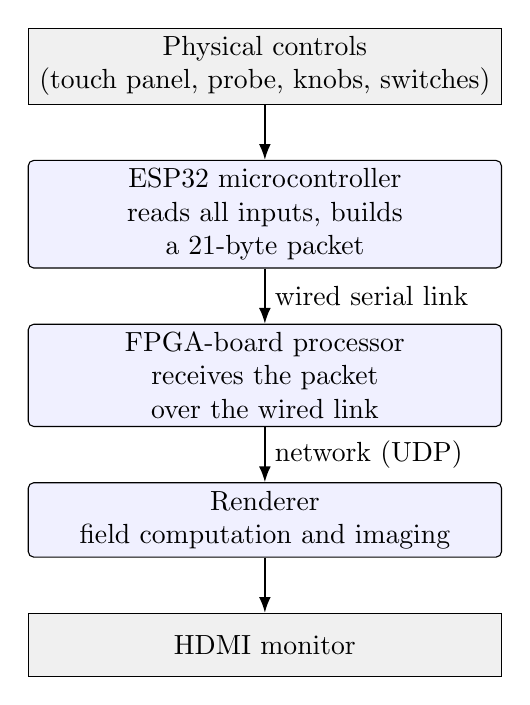
\begin{tikzpicture}[node distance=7mm]
  \node[io, text width=58mm] (ctrl) {Physical controls\\(touch panel, probe, knobs, switches)};
  \node[blk, text width=58mm, below=of ctrl] (esp) {ESP32 microcontroller\\reads all inputs, builds a 21-byte packet};
  \node[blk, text width=58mm, below=of esp] (ps)  {FPGA-board processor\\receives the packet over the wired link};
  \node[blk, text width=58mm, below=of ps]  (rnd) {Renderer\\field computation and imaging};
  \node[io,  text width=58mm, below=of rnd] (mon) {HDMI monitor};
  \draw[arr] (ctrl) -- (esp);
  \draw[arr] (esp)  -- node[right]{wired serial link} (ps);
  \draw[arr] (ps)   -- node[right]{network (UDP)} (rnd);
  \draw[arr] (rnd)  -- (mon);
\end{tikzpicture}
\caption{Data path of the demonstrator within the wider system. This chapter covers the top two blocks; everything below the serial link belongs to the other teams.}
\label{fig:flow}
\end{figure}

% ----------------------------------------------------------------------
\section{The user interface}

All controls sit on one front face (Table~\ref{tab:controls}): one touch surface, four switches and seven rotary knobs. The field-type control is a knob read as three zones, because no three-position switch was available --- a small example of designing around the parts on hand. Every value is sent \emph{normalised} (a fraction of full travel), which makes the controls reusable across both modes; only the Mode-1 probe carries a real measured voltage.

\begin{table}[ht]
\centering
\renewcommand{\arraystretch}{1.2}
\begin{tabularx}{\textwidth}{@{}>{\raggedright\arraybackslash}p{3.3cm} >{\raggedright\arraybackslash}p{2.4cm} >{\raggedright\arraybackslash}X@{}}
\toprule
\textbf{Control} & \textbf{Type} & \textbf{Function} \\
\midrule
Touch panel & 4-wire resistive & $XY$ position (both modes) \\
Mode & switch & Mode 1 / Mode 2 \\
2D/3D & switch & flat or rendered-surface display \\
Wall/Source & switch & what a stylus press places (Mode 2) \\
Clear & switch & wipe the scene; set at power-up to recalibrate \\
Amplitude & knob & source amplitude (Mode 2) \\
Conductivity & knob & wave speed (Mode 2) \\
Field type & knob (3 zones) & show $E$, $B$ or Poynting (Mode 2) \\
Yaw, Pitch, Zoom, Z-scale & 4 knobs & 3D camera view \\
\bottomrule
\end{tabularx}
\caption{The front-panel controls.}
\label{tab:controls}
\end{table}

\begin{figure}[ht]
\centering
\figplaceholder{annotated photograph or drawing of the front panel, labelling each of the seven knobs, the four toggle switches and the touch panel in their left-to-right order}
\caption{The front-panel control layout. \emph{(Insert annotated image.)}}
\label{fig:panel}
\end{figure}

% ----------------------------------------------------------------------
\section{Power supply and analog conditioning}

The whole subsystem runs from the single 5\,V USB feed it shares with the FPGA board (which also ties their grounds together); the board's regulator makes the 3.3\,V from it. The three rails are listed in Table~\ref{tab:rails}.

The seven knobs are referenced directly to the board's regulated \textbf{3.3\,V (3V3) pin}: each is a potentiometer between 3V3 and ground feeding an analog input, so full rotation spans the converter's full range. The pots together draw only a few milliamps, so the pin holds its voltage and no buffered reference rail is needed. The switches simply pull their pin to ground, held high otherwise by internal pull-ups.

\begin{table}[ht]
\centering
\renewcommand{\arraystretch}{1.25}
\begin{tabularx}{\textwidth}{@{}>{\raggedright\arraybackslash}p{3.3cm} >{\raggedright\arraybackslash}X >{\raggedright\arraybackslash}X@{}}
\toprule
\textbf{Rail} & \textbf{Where it comes from} & \textbf{What it feeds} \\
\midrule
$+5$\,V & USB supply (shared with the FPGA) & the probe op-amp's positive supply; the centre copper-tape pad of the conducting sheet \\
3.3\,V & the microcontroller's on-board 3V3 pin & the top end of all seven knobs \\
Ground & common to everything & microcontroller, op-amp, touch panel, the copper-tape border (all four edges) of the conducting sheet, and the FPGA board \\
\bottomrule
\end{tabularx}
\caption{The three supply rails of the control subsystem.}
\label{tab:rails}
\end{table}

Mode 1 adds one analog block, a \textbf{probe buffer} (Figure~\ref{fig:afe}). A unity-gain op-amp follower reads the sheet at near-infinite input impedance, so the probe does not load the field; a resistor divider then scales the probe's $0$--$5$\,V down into the converter's $0$--$3.3$\,V window, and a pull-down holds a lifted probe at a definite zero.

\begin{figure}[ht]
\centering
\resizebox{\textwidth}{!}{%
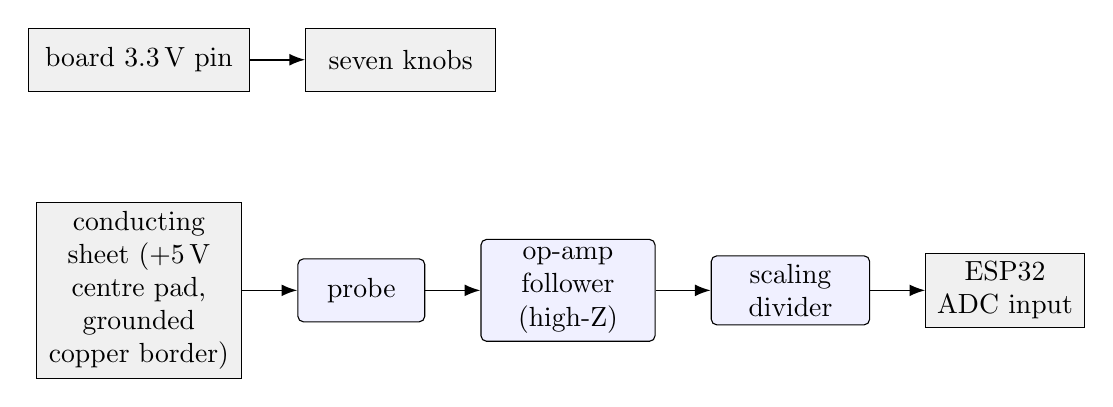
\begin{tikzpicture}[node distance=6mm and 7mm]
  % control reference (top): knobs straight off the board's 3.3 V pin
  \node[io, text width=26mm] (v33) {board 3.3\,V pin};
  \node[io, text width=22mm, right=of v33] (knb) {seven knobs};
  \draw[arr] (v33)--(knb);
  % probe chain (bottom)
  \node[io,  text width=24mm, below=14mm of v33] (sheet) {conducting sheet ($+5$\,V centre pad, grounded copper border)};
  \node[blk, text width=14mm, right=of sheet] (prb)  {probe};
  \node[blk, text width=20mm, right=of prb]   (op2)  {op-amp follower (high-Z)};
  \node[blk, text width=18mm, right=of op2]   (div2) {scaling divider};
  \node[io,  text width=18mm, right=of div2]  (adc)  {ESP32 ADC input};
  \draw[arr] (sheet)--(prb); \draw[arr] (prb)--(op2);
  \draw[arr] (op2)--(div2);  \draw[arr] (div2)--(adc);
\end{tikzpicture}}
\caption{The analog front end. Top: the seven knobs are referenced directly to the board's 3.3\,V pin. Bottom: the probe signal chain for Mode 1, whose unity-gain follower presents a high impedance so the probe does not load the conducting sheet.}
\label{fig:afe}
\end{figure}

Each sub-circuit was verified in SPICE before assembly.

% ----------------------------------------------------------------------
\section{The microcontroller and the control link}

The subsystem is built around an \textbf{ESP32}: a cheap module with a multi-channel analog-to-digital converter, ample I/O, a hardware serial port and Arduino tooling. It does no physics --- it only reads the controls and reports them. Its radio stays off (enabling it would disable a bank of the analog inputs in use), and no analog-output (DAC) pins are used --- the panel is driven with plain digital levels, and calibration absorbs the small offset.

Twenty of the roughly two dozen usable pins are occupied (Table~\ref{tab:pins}). This effectively fills the chip: a couple of controls sit on an input-only pin and on two start-up (``strapping'') pins, all checked to be harmless, so the board is at the practical limit of a single chip --- a fact that drove the design evolution in Section~6.7.

\begin{table}[ht]
\centering
\renewcommand{\arraystretch}{1.25}
\begin{tabularx}{\textwidth}{@{}>{\raggedright\arraybackslash}p{3.1cm} >{\raggedright\arraybackslash}X@{}}
\toprule
\textbf{Pins} & \textbf{Purpose} \\
\midrule
six pins & touch panel --- two axis-drive pairs plus two sense lines (Section~6.5) \\
one input pin & probe voltage (Mode 1) \\
seven analog inputs & the seven knobs: amplitude, conductivity, field-type, yaw, pitch, zoom, vertical scale \\
four digital inputs & mode, 2D/3D, wall/source and clear switches \\
two serial pins & transmit and receive for the link to the FPGA board \\
\bottomrule
\end{tabularx}
\caption{How the twenty occupied pins are allocated.}
\label{tab:pins}
\end{table}

The firmware repeats a fixed cycle about fifty times a second (Figure~\ref{fig:loop}), packing everything into a fixed \textbf{21-byte packet} with a start marker and a checksum (Table~\ref{tab:packet}). This layout is the stable contract with the FPGA team and did not change across hardware revisions. When no touch is valid the position bytes are zero and a flag tells the receiver to place nothing that frame. The ESP32 cannot send UDP itself (its radio is off), so the packet goes by wire to the FPGA board's processor, which forwards it onto the network to the renderer (Figure~\ref{fig:flow}).

\begin{figure}[ht]
\centering
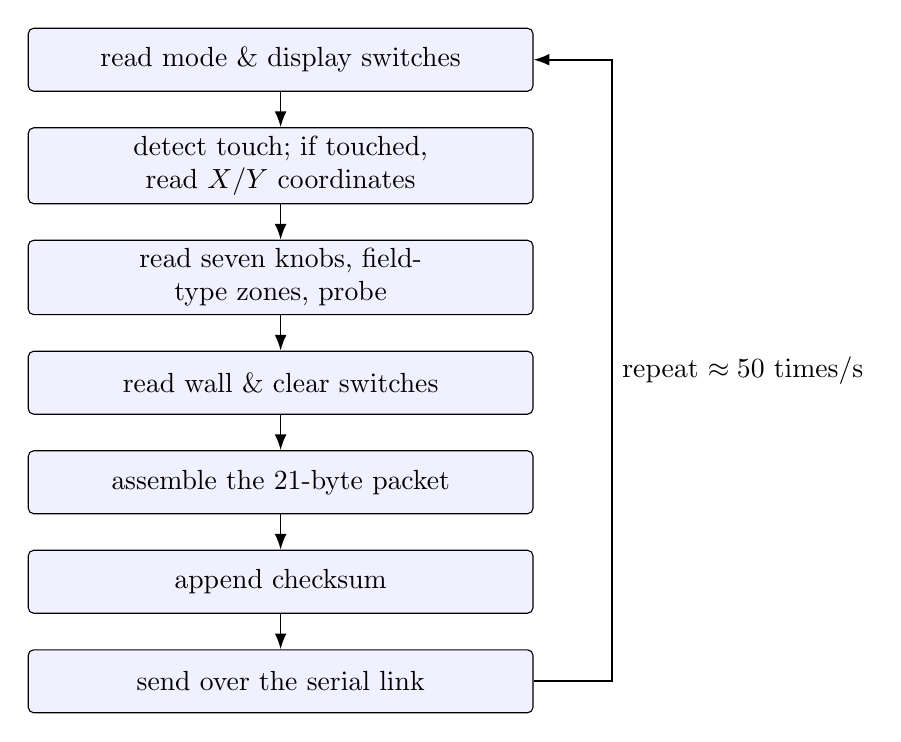
\begin{tikzpicture}[node distance=4.5mm]
  \node[blk, text width=62mm] (a) {read mode \& display switches};
  \node[blk, text width=62mm, below=of a] (b) {detect touch; if touched, read $X$/$Y$ coordinates};
  \node[blk, text width=62mm, below=of b] (c) {read seven knobs, field-type zones, probe};
  \node[blk, text width=62mm, below=of c] (d) {read wall \& clear switches};
  \node[blk, text width=62mm, below=of d] (e) {assemble the 21-byte packet};
  \node[blk, text width=62mm, below=of e] (f) {append checksum};
  \node[blk, text width=62mm, below=of f] (g) {send over the serial link};
  \draw[arr] (a)--(b); \draw[arr] (b)--(c); \draw[arr] (c)--(d);
  \draw[arr] (d)--(e); \draw[arr] (e)--(f); \draw[arr] (f)--(g);
  \draw[arr] (g.east) -- ++(10mm,0) |- node[right, pos=0.25]{repeat $\approx 50$ times/s} (a.east);
\end{tikzpicture}
\caption{The fixed firmware cycle, repeated about fifty times per second.}
\label{fig:loop}
\end{figure}

\begin{table}[ht]
\centering
\renewcommand{\arraystretch}{1.25}
\begin{tabularx}{\textwidth}{@{}>{\raggedright\arraybackslash}p{2.6cm} >{\raggedright\arraybackslash}X@{}}
\toprule
\textbf{Bytes} & \textbf{Contents} \\
\midrule
1 & start marker (a fixed recognisable byte) \\
1 & flags: experiment, 2D/3D, field type, wall-or-source, clear active, touch valid \\
$2+2$ & touch position, as a column and row on the display grid \\
2 & source amplitude \\
2 & conductivity (wave speed) \\
2 & probe voltage (Mode 1) \\
$2+2+2+2$ & the four camera-view knobs: yaw, pitch, zoom, vertical scale \\
1 & checksum over the message body \\
\bottomrule
\end{tabularx}
\caption{The fixed twenty-one-byte control packet.}
\label{tab:packet}
\end{table}

% ----------------------------------------------------------------------
\section{The touch panel: sensing and calibration}

Getting clean, trustworthy coordinates from the panel took more effort than any other part.

\textbf{How it works.} The panel is two resistive layers held a hair apart; a press shorts them at the contact point (Figure~\ref{fig:touch}). Position is read by driving one layer as a voltage ramp and sensing the contact voltage on the floating layer, swapping the layers for the two axes --- three short phases per loop (Table~\ref{tab:phases}).

\begin{figure}[ht]
\centering
\figplaceholder{diagram of the four-wire panel: the two conductive layers, the edge electrodes, and the two measurement phases showing how the horizontal and vertical positions are read in turn}
\caption{Reading a four-wire resistive panel. \emph{(Insert diagram.)}}
\label{fig:touch}
\end{figure}

\begin{table}[ht]
\centering
\footnotesize
\renewcommand{\arraystretch}{1.2}
\begin{tabularx}{\textwidth}{@{}>{\raggedright\arraybackslash}p{2.2cm} >{\raggedright\arraybackslash}X >{\raggedright\arraybackslash}X >{\raggedright\arraybackslash}p{2.0cm}@{}}
\toprule
\textbf{Phase} & \textbf{Layer driven} & \textbf{Sensed on} & \textbf{Result} \\
\midrule
Touch detect & Y- pulled low & X+ via pull-up & pressed? \\
Read X & X layer (X+ high, X- low) & a Y terminal & $X$ position \\
Read Y & Y layer (Y+ high, Y- low) & an X terminal & $Y$ position \\
\bottomrule
\end{tabularx}
\caption{The three read phases of the four-wire panel.}
\label{tab:phases}
\end{table}

\textbf{Clean coordinates.} Each axis is sensed on a dedicated low-leakage input, so the high-impedance contact node stays linear, and read with the converter's millivolt calibration. Readings are filtered --- a median for touch detection, a trimmed mean of a dozen samples per coordinate --- after a short settling pause. \textbf{Orientation} (axis swaps and mirroring) is always corrected in software, never by rewiring.

\textbf{Calibration.} The corners never read the true extremes, so the user sets the range with a quick \textbf{two-corner} press --- one corner, then the opposite --- and only firm presses are learned. The range is saved to non-volatile memory and reloaded at boot, and can be redone by holding the clear switch at power-up. Each press is then converted as in Figure~\ref{fig:pipeline}, and the finished grid cell goes straight into the packet.

\begin{figure}[ht]
\centering
\resizebox{\textwidth}{!}{%
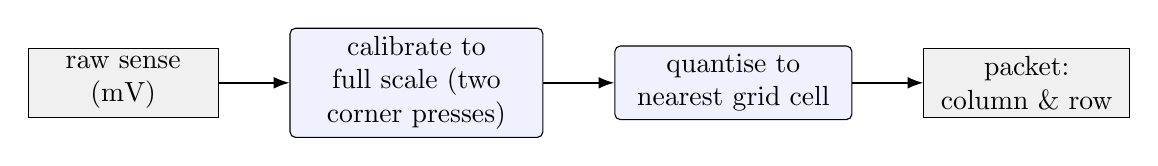
\begin{tikzpicture}[node distance=9mm]
  \node[io,  text width=22mm] (raw) {raw sense (mV)};
  \node[blk, text width=30mm, right=of raw]  (cal)  {calibrate to full scale (two corner presses)};
  \node[blk, text width=28mm, right=of cal]  (grid) {quantise to nearest grid cell};
  \node[io,  text width=24mm, right=of grid] (pkt)  {packet: column \& row};
  \draw[arr] (raw)--(cal); \draw[arr] (cal)--(grid); \draw[arr] (grid)--(pkt);
\end{tikzpicture}}
\caption{Touch-coordinate pipeline: each raw reading is calibrated, quantised to a display-grid cell, and sent in the packet.}
\label{fig:pipeline}
\end{figure}

% ----------------------------------------------------------------------
\section{Enclosure and mechanical design (box modelling)}

A showcase demonstrator needs a real housing, so a custom enclosure was modelled and 3D-printed, evolving toward the same simplicity as the electronics. It is a single \textbf{open-bottomed cover} --- an upturned tray --- that drops over the baseboard-mounted electronics: no internal fixings, a clean screwless top face, the FPGA left open in its bay, and nothing to trap heat. Its key features are listed in Table~\ref{tab:box} and its top-face layout in Figure~\ref{fig:box-top}.

\begin{table}[ht]
\centering
\renewcommand{\arraystretch}{1.25}
\begin{tabularx}{\textwidth}{@{}>{\raggedright\arraybackslash}p{3.6cm} >{\raggedright\arraybackslash}X@{}}
\toprule
\textbf{Feature} & \textbf{Size / detail} \\
\midrule
Overall cover (W$\times$D$\times$H) & $318 \times 172 \times 55$\,mm \\
Walls / top plate & 3\,mm / 5\,mm \\
Touch-panel window & stepped recess + lip, back-left; conducting sheet lies on top in Mode 1 \\
FPGA bay & $\sim$120 $\times$ 90\,mm open cut-out, back-right (HDMI/USB/buttons stay exposed) \\
Control strip & front row of 11 holes --- 7 knobs (7\,mm dia.) and 4 toggle switches \\
Cable slot & $\sim$40 $\times$ 22\,mm, back wall \\
Companion parts & panel frame (bezel) + paper frame (holds the conducting sheet flat) \\
\bottomrule
\end{tabularx}
\caption{Key features of the 3D-printed cover.}
\label{tab:box}
\end{table}

The neatest detail is the panel mount: the panel drops into a shallow stepped recess and rests on a thin internal lip, leaving its active area exposed through a window while its bezel sits flush with the top. Two small companion parts make one panel serve both modes (Figure~\ref{fig:box-frames}): a slim \textbf{panel frame} clamps the touch panel into that recess, and a \textbf{paper frame} holds the floppy conducting sheet flat over the same window for Mode 1.

\begin{figure}[ht]
\centering
\figplaceholder{the dimensioned top-view layout of the cover, marking the panel window, the FPGA bay, the eleven-hole control strip and the rear cable slot}
\caption{Top-view layout of the cover. \emph{(Insert dimensioned drawing.)}}
\label{fig:box-top}
\end{figure}

\begin{figure}[ht]
\centering
\figplaceholder{photographs of the printed panel frame and paper frame, ideally one showing the conducting sheet held flat in the paper frame over the panel}
\caption{The printed panel frame and paper frame. \emph{(Insert photographs.)}}
\label{fig:box-frames}
\end{figure}

The model is \textbf{parametric} --- every dimension is a named value, so a single edit regenerates a consistent model if a part size changes --- and was kept in more than one CAD tool sharing the same values. It is printed \textbf{upside-down} so every opening forms with no overhangs and needs no supports (PLA or PETG). At 318\,mm it exceeds a typical print bed, so it is split into two halves joined at a seam; the finished enclosure is therefore two box parts plus the two frames. Boards mount to the baseboard, the framed panel and the knobs and switches fit the top face, the halves join, and the cover drops over with cables exiting the rear slot. Being a simple cover it has no internal standoffs and a single panel window --- exactly what the final one-panel design needs.

\begin{figure}[ht]
\centering
\figplaceholder{a photograph of the printed enclosure, ideally showing the two halves joined and the whole console assembled with the panel, knobs and FPGA in place}
\caption{The printed and assembled enclosure. \emph{(Insert photograph.)}}
\label{fig:box-printed}
\end{figure}

% ----------------------------------------------------------------------
\section{Design evolution: how the hardware reached its final form}

The subsystem reached its final form over three iterations (Figure~\ref{fig:evolution}, Table~\ref{tab:compare}), each trading complexity for simplicity without losing capability.

\begin{figure}[ht]
\centering
\resizebox{\textwidth}{!}{%
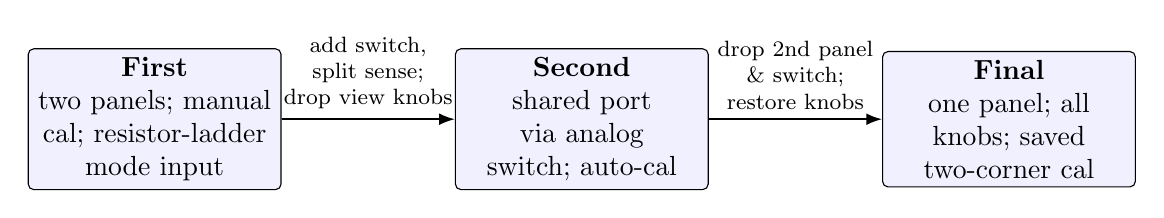
\begin{tikzpicture}[node distance=22mm]
  \node[blk, text width=30mm] (v1) {\textbf{First}\\two panels; manual cal; resistor-ladder mode input};
  \node[blk, text width=30mm, right=of v1] (v2) {\textbf{Second}\\shared port via analog switch; auto-cal};
  \node[blk, text width=30mm, right=of v2] (v3) {\textbf{Final}\\one panel; all knobs; saved two-corner cal};
  \draw[arr] (v1) -- node[above, align=center, font=\footnotesize]{add switch,\\split sense;\\drop view knobs} (v2);
  \draw[arr] (v2) -- node[above, align=center, font=\footnotesize]{drop 2nd panel\\\& switch;\\restore knobs} (v3);
\end{tikzpicture}}
\caption{The three hardware iterations: each step sheds complexity while keeping --- and finally restoring --- capability.}
\label{fig:evolution}
\end{figure}

\textbf{First --- two panels.} One panel per experiment, the full seven knobs, mode and display packed onto one input through a resistor ladder, and calibration typed in by hand. The richest features and the fewest extra parts, but the pin budget was at its limit, the wiring was busy, and reusing one pin for both drive and sense slightly bowed the coordinates.

\textbf{Second --- shared port.} Since only one panel is ever live, an analog switch routes one clean six-wire port to the active panel; separate drive and sense lines linearised the coordinates, the resistor ladder became two plain switches, and calibration became automatic. To fit the pins, the four camera-view knobs were dropped --- and it still carried two panels and an extra chip.

\textbf{Final --- one panel.} Because the modes never run together and both only need an $XY$, a single panel serves both (the sheet lies on it in Mode 1). That deleted the second panel and the switch, restored all seven knobs, and made calibration a persistent two-press routine --- at the cost of a fully used pin budget.

\begin{table}[ht]
\centering
\footnotesize
\renewcommand{\arraystretch}{1.3}
\begin{tabularx}{\textwidth}{@{}>{\raggedright\arraybackslash}p{2.7cm}
  >{\raggedright\arraybackslash}X
  >{\raggedright\arraybackslash}X
  >{\raggedright\arraybackslash}X@{}}
\toprule
\textbf{Aspect} & \textbf{First design} & \textbf{Second design} & \textbf{Final design} \\
\midrule
Touch panels & two, independent & two, sharing one wiring set & one, serves both experiments \\
Extra components for the panel & none & an analog switch chip & none \\
Mode / display selection & one shared input, resistor-ladder coded & two plain switches & two plain switches \\
Knobs fitted & seven (full set) & three (camera knobs dropped) & seven (full set restored) \\
Coordinate quality & slightly bowed (shared drive/sense) & linear (separate drive/sense) & linear (separate drive/sense) \\
Calibration & manual, typed in & automatic, redone each power-up & two-press, saved permanently \\
Pin usage & at the limit & comfortable & at the limit \\
Mechanical complexity & highest & high & lowest \\
\bottomrule
\end{tabularx}
\caption{The three hardware iterations compared.}
\label{tab:compare}
\end{table}

In short, the design moved from many features at the cost of complexity, through cleaner wiring at the cost of features, to a final form that \textbf{recovered the full feature set while being the simplest of the three}.

% ----------------------------------------------------------------------
\section{Summary}

The demonstrator makes the invisible physics graspable: through one touch surface, four switches and seven knobs, a user can measure a real electrostatic field on a conducting sheet and watch the simulation agree with it, or paint sources and walls and watch waves propagate. Behind the interface, the knobs reference the board's own 3.3\,V pin and a high-impedance amplifier conditions the Mode-1 probe, all read by a single ESP32 that streams a compact, checksummed packet by wire into the rest of the system. The touch panel --- the fussiest element --- is made trustworthy by linear sensing, filtering, software-corrected orientation, and a calibration the demonstrator remembers. Everything is housed in a parametric, support-free 3D-printed cover that splits to fit an ordinary printer. The path from a two-panel prototype to the final one-panel console captures the subsystem's guiding idea: do the most for the user with the least to go wrong.

\end{document}
